\documentclass[titlepage]{jsarticle}

\usepackage{color}
\usepackage[dvips]{graphicx}
\usepackage{listings}

\title{コンピュータグラフィックス基礎 課題2}
\author{201111365 坂口和彦}

\lstdefinestyle{program}{
  basicstyle=\small\tt,
  keywordstyle=\bf,
  identifierstyle=,
  commentstyle=,
  stringstyle=,
  emphstyle=,
  backgroundcolor=\color[gray]{0.8},
  language=C,
  frame=trbl,
  rulecolor=\color{white},
  numbers=left,
  numberstyle=,
  basewidth={0.54em, 0.45em},
  lineskip=-0.2zw
}

\renewcommand{\lstlistingname}{リスト}

\begin{document}

\maketitle

\section{課題2-1}

直線を描画する関数と、$\frac{1}{8}$円を描画する関数を実装した。ソースコードをリスト\ref{list:impl1}に示す。

\begin{lstlisting}[style=program, label=list:impl1, caption=課題2-1のソースコード]
void line(int x1, int y1, int x2, int y2)
{
    int x = x1, y = y1, e = 0;
    while(1){
        ploti(x, y);
        x++;
        e += y2-y1;
        if(x2-x1 <= e){
            e -= x2-x1;
            y++;
        }
        if(x == x2) break;
    }
}

void octant(int r)
{
    int x = 0, y = r, d = 3 - 2*r;
    while(1){
        ploti(x, y);
        if(d < 0){
            d += 6+4*x;
        }
        else{
            d += 10+4*x-4*y;
            y--;
        }
        x++;
        if(y < x) break;
    }
}
\end{lstlisting}

このプログラムの実行結果を図\ref{fig:output1}に示す。

\begin{figure}[htbp]
\begin{center}

\includegraphics[width = 150mm]{1.ps}
\end{center}
\caption{課題2-1の実行結果}
\label{fig:output1}
\end{figure}

図を見て分かる通り、直線と円弧が描けた。

\section{課題2-2}

直線を描画する関数と、円を描画する関数を実装した。リスト\ref{list:impl2}にソースコードを示す。

\begin{lstlisting}[style=program, label=list:impl2, caption=課題2-2のソースコード]
#define SWAP(type, a, b) do { type tmp = a; a = b; b = tmp; } while(0)

void  ploti(int x, int y)
{ glBegin(GL_POINTS); glVertex2i(x,y); glEnd(); }

void  linei(int x1, int y1, int x2, int y2)
{
    int f1, f2, f3, x = 0, y = 0, e = 0;
    if(f1 = (x2 <= x1)){
        SWAP(int, x1, x2);
    }
    if(f2 = (y2 <= y1)){
        SWAP(int, y1, y2);
    }
    if(f3 = (x2 - x1 <= y2 - y1)){
        SWAP(int, x1, y1);
        SWAP(int, x2, y2);
    }
    while(1){
        int rx = f1 ? x2 - x : x1 + x, ry = f2 ? y2 - y : y1 + y;
        if(f3) ploti(ry, rx);
        else ploti(rx, ry);
        x++;
        e += y2-y1;
        if(x2-x1 <= e){
            e -= (x2 - x1);
            y++;
        }
        if(x == x2 - x1) break;
    }
}

void  circlei(int x, int y, int r)
{
    int cx = 0, cy = r, d = 3 - 2*r;
    while(1){
        ploti(x+cx, y+cy);
        ploti(x+cx, y-cy);
        ploti(x-cx, y+cy);
        ploti(x-cx, y-cy);
        ploti(x+cy, y+cx);
        ploti(x+cy, y-cx);
        ploti(x-cy, y+cx);
        ploti(x-cy, y-cx);
        if(d < 0){
            d += 6+4*cx;
        }
        else{
            d += 10+4*cx-4*cy;
            cy--;
        }
        cx++;
        if(cy < cx) break;
    }
}
\end{lstlisting}

このプログラムの実行結果を図\ref{fig:output2}に示す。

\begin{figure}[htbp]
\begin{center}
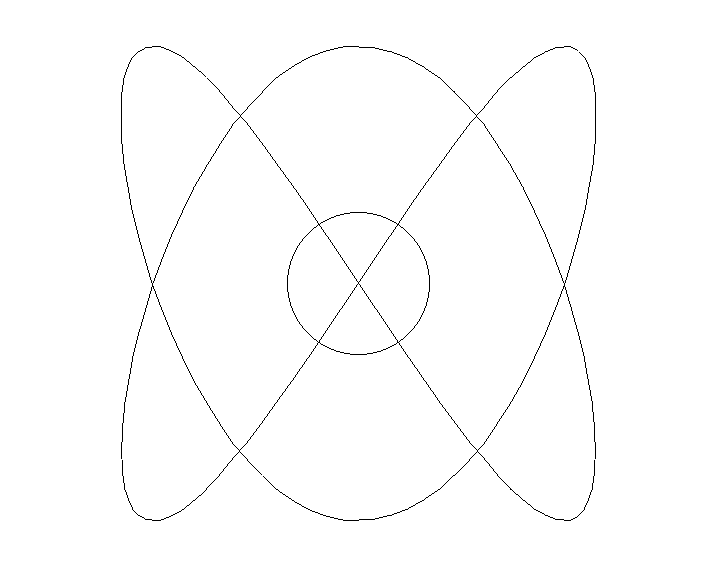
\includegraphics[width = 150mm]{2.ps}
\end{center}
\caption{課題2-2の実行結果}
\label{fig:output2}
\end{figure}

図を見て分かる通り、直線と円が描けた。

\section{工夫/苦労した点、感想等}

実装を短くするため、課題2-2では \texttt{SWAP} マクロを用いた。

\end{document}

